%BEGIN: Simulation of Smart Environments
\section{Simulation of Smart Environments}\label{sec:sim_of_smart_envs}

Armac and Retkowitz developed a tool called \emph{eHomeSimulator}, which was build in order to support the simulation of smart environments, or as the authors refer to them in the present work \emph{eHomes} \cite{armac2007simulation}. The motivation behind the work is that smart environments constitute already an important research area, but building a real eHome is associated with high effort and financial costs. Therefore, the eHomeSimulator helps in abstracting out from creating buildings (the actual physical environment) and purchasing devices, allowing the researcher to focus only on software engineering aspects and challenges involved in eHome development (e.g. developing services, deployment, etc).\\

Describing in details the eHome is out of scope, but for clarity, we will a offer a short description. eHome is basically a framework consisting of a hardware platform (the residential gateway) and a software platform (service gateway, runs on top of the hardware platform). The devices and appliances, which make up the eHome, are connected to the hardware platform. They are of two basic types: sensors and actuators. Sensors offer contextual information like temperature, humidity, etc; while actuators can change the environment's state (e.g. a speaker, a heater). The hardware platform is governed by the software platform which acts as a runtime environment for eHome services. These services can be of two types: basic and integrating. Basic service are meant to control devices (e.g. a lamp driver) while the integrating services are composed of various basic service. These services are developed based on the OSGi component model \cite{allianceosgi}, imposing a highly decoupled architecture to the service model and offering high reusability of the developed services.\\

The eHomeSimulator was built on top of the eHome framework to allow intuitive interaction and to visually represent the state of the simulated environment. In the evaluation process of the simulator, eHome environments consisted of three main elements: rooms, devices and persons (agents interacting with the environment). The graphical representation was a 2D view with a view point from top, which is built up from three layers:
\begin{itemize}
	\item The bottom layer contains the graphics to represent the background (floor, walls and furniture) build up from tiles placed one next to each other.
	\item On top of the background, there is the middle layer representing the graphics of the devices. These are only static devices and they can have different colours based on their state.
	\item The top layer represents the agents interacting with the environment. They can move freely in all accessible areas, interacting with the devices.
\end{itemize}

There is an environment editor which assists in setting up a simulated environment. The process starts by designing the room, walls and furniture using Google Sketchup\footnote{\url{http://www.sketchup.com}} which then is uploaded into the editor. On top of this base we can further place the devices and appliances.\\

The eHomeSimulator's architecture is based on the Model View Controller design pattern \cite{erich1995design}. The model of the system holds the data structures representing the current state of the system, the view implements the graphical representation based on the current model and the controller process the user interaction with the simulator, updating the view according to changes in the model.\\

The image depicted in Figure \ref{fig:simulated_env} displays a simulation in progress. On the right side, we can observe the agent interacting with the environment while on the left side there is a control panel displaying contextual data of the monitored entities and allows to interact with nearby devices (e.g. turn on/off a lamp).

\begin{figure}[H]
	\centering
	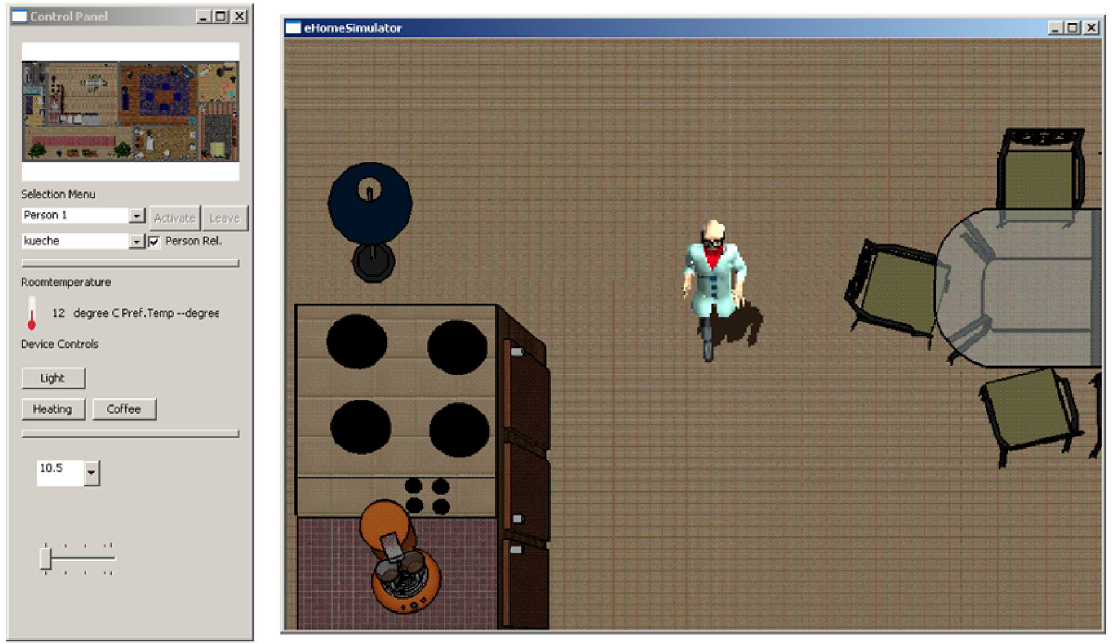
\includegraphics[width=\linewidth]{gfx/Chapter2/simulated_env}
	\caption{The GUI of eHomeSimulator}
	\label{fig:simulated_env}
\end{figure}

The framework allows to simulate only sensors and devices. Physical objects are passive and unidentifiable, they are part of the first layer, the bottom layer containing the graphics to represent the background (floor, walls and furniture).\\

As for interacting with the simulated environment, the user can manipulate the agent (the virtual avatar), to walk around in the 2D environment. Given the nature of the visualization, the agent can be facing four directions: forward, backward, left or right. Sensor and devices are activated on a per room basis, not on actual proximity to each individual entity. Devices in the current room can be operated through the \emph{Control Panel} (e.g. turn lamp on/off).\\
%END: Simulation of Smart Environments